\documentclass[12pt,twoside,a4paper]{report}
\usepackage[a4paper,width=150mm,top=25mm,bottom=25mm,bindingoffset=6mm]{geometry}

\usepackage[utf8x]{inputenc}
\usepackage[slovak]{babel}
\usepackage{palatino,verbatim}

% Balicek pre priamu rec - \say
\usepackage{dirtytalk}

% Balicek "alltt" je to iste ako "verbatim" mod, ale navyse podporuje aj formatovacie znacky textu
\usepackage{alltt}

% Obrazky
\usepackage{graphicx}
\graphicspath{ {obr/} }

% Cislovanie obrazkov a tabuliek
\usepackage{chngcntr}
%Cisluj obrazky nezavisle od cisla kapitol/podkapitol
\counterwithout{figure}{subsection}
\counterwithout{table}{subsection}

% Referencovanie kapitol/sekcii/... podľa ich nadpisu
\usepackage{nameref}

% Tabulky s viacriadkovymi bunkami a zlucenymi bunkami
% Tabulky generujem naastrojom "http://www.tablesgenerator.com/"
\usepackage{booktabs}
\usepackage{multirow}
% LaTeX ma problemy s prikazmi cline a cmidrule, ked je babel nastaveny na slovencinu/cestinu, kvoli definicii pomlcky
\usepackage{etoolbox}
\preto\tabular{\shorthandoff{-}}

%Uloz obrazok tam, kde je deklarovany
%\usepackage[subsection]{placeins}

\newcommand\sktxt[1]{\foreignlanguage{slovak}{#1}}

\begin{document}
\pagenumbering{arabic}

\setcounter{chapter}{1}
\chapter*{Distribúcia multicastovej prevádzky}
\paragraph{}
Andrej Šišila, Marián Vachalík

\tableofcontents

\newpage
\section{Topológia}
\paragraph{}
Budeme konfigurovať distribúciu multicastovej prevádzky so smerovacím protokolom IS-IS na topológií, ktorá je znázornená na obrázku \ref{fig:mcast_isis_topo}. IP adresácia je uvedená v tabuľke \ref{tab:ip_adresacia} a dopĺňa grafické znázornenie topológie na obrázku \ref{fig:mcast_isis_topo}.

\begin{figure}[!htb]
\centering
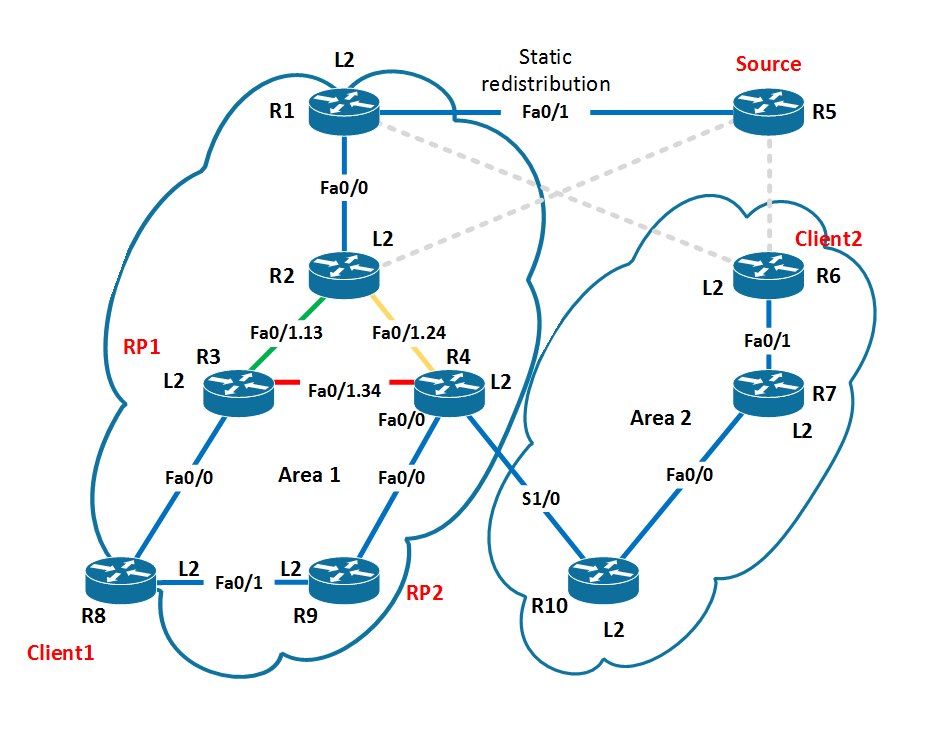
\includegraphics[width=12cm,keepaspectratio]{mcast_isis_topo}
\caption{Topológia IS-IS}
\label{fig:mcast_isis_topo}
\end{figure}



\begin{table}[!htb]
\centering
\caption{IP adresácia}
\label{tab:ip_adresacia}
\begin{tabular}{|c|c|l|l|l|}
\hline
\multicolumn{1}{|c|}{\textbf{Smerovač}}    & \multicolumn{1}{c|}{\textbf{Funkcia}}                        & \multicolumn{1}{c|}{\textbf{Rozhranie}} & \multicolumn{1}{c|}{\textbf{IP adresa}} & \multicolumn{1}{c|}{\textbf{Maska}} \\ \hline
\multirow{3}{*}{R1}  & \multirow{3}{*}{L2}                   & Fa0/0                                   & 10.0.12.1                               & 255.255.255.0                       \\ \cline{3-5} 
                     &                                         & Fa0/1                                   & 10.100.15.1                             & 255.255.255.0                       \\ \cline{3-5} 
                     &                                         & Lo0                                     & 10.255.255.1                            & 255.255.255.255                     \\ \hline
\multirow{3}{*}{R2}  & \multirow{3}{*}{L2}             & Fa0/0                                   & 10.0.12.2                               & 255.255.255.0                       \\ \cline{3-5} 
                     &                                         & Fa0/1                                   & 10.100.234.2                             & 255.255.255.0                       \\ \cline{3-5}
                     &                                         & Lo0                                     & 10.255.255.2                            & 255.255.255.255                     \\ \hline
\multirow{4}{*}{R3}  & \multirow{4}{*}{L1/L2}                    & Fa0/0                                   & 10.1.38.3                               & 255.255.255.0                       \\ \cline{3-5} 
                     &                                         & Fa0/1                                   & 10.0.234.3                              & 255.255.255.0                       \\ \cline{3-5} 
                     &                                         & S1/0                                    & 10.2.39.3                               & 255.255.255.252                     \\ \cline{3-5} 
                     &                                         & Lo0                                     & 10.255.255.3                            & 255.255.255.255                     \\ \hline
\multirow{4}{*}{R4}  & \multirow{4}{*}{L1/L2}                    & Fa0/0                                   & 10.2.49.4                               & 255.255.255.0                       \\ \cline{3-5} 
                     &                                         & Fa0/1                                   & 10.0.234.4                              & 255.255.255.0                       \\ \cline{3-5} 
                     &                                         & S1/0                                    & 10.3.104.4                              & 255.255.255.252                     \\ \cline{3-5} 
                     &                                         & Lo0                                     & 10.255.255.4                            & 255.255.255.255                     \\ \hline
\multirow{2}{*}{R5}  & \multirow{2}{*}{Smerovač iného systému} & Fa0/1                                   & 10.100.15.5                             & 255.255.255.0                       \\ \cline{3-5} 
                     &                                         & Lo0                                     & 10.255.255.5                            & 255.255.255.255                     \\ \hline
\multirow{2}{*}{R6}  & \multirow{2}{*}{L1}             & Fa0/0                                   & 10.4.67.6                               & 255.255.255.0                       \\ \cline{3-5} 
                     &                                         & Lo0                                     & 10.255.255.6                            & 255.255.255.255                     \\ \hline
\multirow{3}{*}{R7}  & \multirow{3}{*}{L1}             & Fa0/1                                   & 10.4.67.7                               & 255.255.255.0                       \\ \cline{3-5} 
                     &                                         & S1/1                                    & 10.4.107.7                              & 255.255.255.0                       \\ \cline{3-5} 
                     &                                         & Lo0                                     & 10.255.255.7                            & 255.255.255.255                     \\ \hline
\multirow{2}{*}{R8}  & \multirow{2}{*}{L1}             & Fa0/0                                   & 10.1.38.8                               & 255.255.255.0                       \\ \cline{3-5} 
                     &                                         & Lo0                                     & 10.255.255.8                            & 255.255.255.255                     \\ \hline
\multirow{3}{*}{R9}  & \multirow{3}{*}{L1}             & Fa0/0                                   & 10.2.49.9                               & 255.255.255.0                       \\ \cline{3-5} 
                     &                                         & S1/0                                    & 10.2.39.9                               & 255.255.255.0                       \\ \cline{3-5} 
                     &                                         & Lo0                                     & 10.255.255.9                            & 255.255.255.255                     \\ \hline
\multirow{3}{*}{R10} & \multirow{3}{*}{L1/L2}                    & S1/0                                    & 10.3.104.10                              & 255.255.255.0                       \\ \cline{3-5} 
                     &                                         & S1/1                                    & 10.4.107.10                              & 255.255.255.0                       \\ \cline{3-5} 
                     &                                         & Lo0                                     & 10.255.255.10                           & 255.255.255.255                     \\ \hline
\end{tabular}
\end{table}


% Novu kapitolu davam na novu stranu, lebo bez toho mi zobrazuje tabulku v dalsej kapitole, kde ale tabulka nepatri.
\newpage


\section{Úlohy}
\subsection{Nakonfigurovať IS-IS}

\end{document}